\documentclass[DM,lsstdraft,authoryear,toc]{lsstdoc}
% lsstdoc documentation: https://lsst-texmf.lsst.io/lsstdoc.html

% Package imports go here.
\usepackage{graphicx}
\usepackage{url}
\usepackage{latexsym}
\usepackage{color}
\usepackage{enumitem}

% Local commands go here.

% To add a short-form title:
% \title[Short title]{Title}
\title[Alerts Latency]{Science Drivers for LSST Alert Distribution Latency}

% Optional subtitle
% \setDocSubtitle{A subtitle}

\author{%
M.~L.~Graham, with contributions from the Transients and Variable Stars Science Collaboration
}

\setDocRef{DMTN-TBD}
\date{\today}
% Optional: name of the document's curator
% \setDocCurator{The Curator of this Document}
\setDocUpstreamLocation{\url{https://github.com/lsst-dm/dmtn-xxx}}

\setDocAbstract{%
\textcolor{red}{\bf EXTREME DRAFT. DO NOT CITE OR READ.}\\
A gathering place for the science drivers related to alert packet distribution latency.
}

% Change history defined here.
% Order: oldest first.
% Fields: VERSION, DATE, DESCRIPTION, OWNER NAME.
% See LPM-51 for version number policy.
\setDocChangeRecord{%
  \addtohist{0}{2019-11-14}{Inception.}{Melissa Graham}
  \addtohist{0.1}{2020-01-09}{Early draft.}{Melissa Graham}
}

\begin{document}

% Cite requirements using these macros.
% \lsrreq \ossreq \dmreq \reqparam 

% Create the title page.
% Table of contents is added automatically with the "toc" class option.
\maketitle

% % % % % % % % % % % % % % % % % % % % % % % % % %
\section{Introduction} \label{sec:intro}

% The LSST Science Requirements Document \citedsp{LPM-17} specifies that information about the detections of transient, variable, and moving objects be released promptly as a data stream.

This document gathers the scientific motivations for --- and impacts of --- the alert distribution timescale, also called the latency.
Alert packets will play a major role in the scientific impact of LSST, in part because they are the only LSST data product that is both world public (exempt from any proprietary period) and publicly accessible, as they are distributed to community brokers and not solely available via the LSST Science Platform (LSP).
Although the contents of the Prompt products database (PPDB) from which alerts are generated are also world public, access to the PPDB is restricted to individuals with data rights \citedsp{LDO-013} who have authenticated accounts in the LSP.

It is a requirement\reqparam{numStreams}\dmreq{0391} that the DMS be capable of supporting the transmission of at least 5 full alert streams within 60 seconds of image readout --- more specifically, that the data management system (DMS) be capable of supporting the distribution of at least 98\%\reqparam{OTT1}\reqparam{OTR1}\lsrreq{0101}\lsrreq{0025}\ossreq{0127}\dmreq{0004} of alerts for each visit within 60 seconds of the end of image readout.
The 60 second latency was broadly scientifically motivated by a desire to explore the parameter space for very short timescale transients and variables which might last only a few minutes \citedsp{LPM-17}.
The number of 5 full streams is based in part on estimates of the alert stream data rate and the bandwidth allocated to alert distribution in the LSST data facility \citedsp{DMTN-102}.

Increasing the alert latency \emph{might} enable the stream to be delivered to more brokers, thereby increasing the amount of alerts-related science done by the community.
Or it might allow human and computational resources that are currently dedicated to building a DMS which can deliver a 1 minute latency to be repurposed. 
\textbf{There is currently no tabled proposal to increase the alert latency from 60 seconds}, but in case there ever is, this document collects the science drivers for short timescale alert distribution.
\textbf{Time-domain astronomy remains a rapidly evolving field and this should be considered a living, in-progress document}.

\subsection{Summary}

This document reports that most alerts-related science goals would be satisfied with a $\sim$5 minute alert timescale, but that the quickly evolving fields of fast radio bursts and gravitational wave events may soon provide more robust motivation for a 60 second latency.

%This draft contains content pertaining to the following open tickets in the DM-SST epic "Studies Around Alerts" (assignees):
%\begin{itemize}
%\item DM-20299, Scientific use-cases requiring $<$5 minute access (Graham)
%\end{itemize}


\clearpage
% % % % % % % % % % % % % % % % % % % % % % % % % %
\section{Science Drivers for Alert Latency} \label{sec:latency}

Generally, for science goals that require alerts on timescales shorter than $\sim$5 minutes, their need stems from targets that are fast-evolving or short-lived (or both) and require follow-up on timescales shorter than $\sim$15--30 minutes.
Since most observing strategies for the WFD main survey do not revisit fields on timescales shorter than $\sim$15 minutes (strategies that do pair visits aim for closer to $\sim$22 minute gaps), brokers must be able to confidently identify such targets with single-epoch single-filter LSST photometry, or be using additional information (e.g., host galaxy characteristics, coincident alerts from other surveys).
For the purposes of this discussion, an optimistic outlook is assumed, and the difficulty in identifying targets with a single epoch of LSST photometry is not considered as a reason to downgrade the importance of a 1 minute alert latency.

\begin{itemize}
\item {\bf A TVS Survey (\S~\ref{ssec:latency_tvs})} found that only $<$10\% of respondents reported that requiring alerts within 1 minute was necessary for their science goals.
\item {\bf GW Follow-up (\S~\ref{ssec:latency_emgw}) ---} Although a 5 minute latency would suffice for kilonovae (days-long optical counterparts to neutron star mergers), some theoretical models predict optical emission within the first hour (e.g., jet break-out or spin-down energy from the merger). However, these GW scientific motivators for a 1 minute alert latency are moot if the time between GW event and LSST ToO imaging remains $\sim$tens of minutes.
\item {\bf Gamma-Ray Bursts (\S~\ref{ssec:latency_grb}) ---} \textcolor{red}{Tentatively,} alerts for the coincident optical counterparts of short GRBs would be most scientifically useful if distributed within 1 minute, but the predicted occurrence rate is $\lesssim$20 over the 10-year LSST survey.
\item {\bf Fast Radio Bursts (\S~\ref{ssec:latency_frb}) ---} \textcolor{red}{Tentatively,} some models predict that a short, bright burst of optical emission from the physical mechanism powering FRBs could be detected by LSST 5 to 15 minutes prior to the radio signal.
If such optical events occur with significant frequency, are bright and consistently detectable, and can be identified with a single-filter detection, and if radio telescopes can respond within minutes, then LSST is the most promising future facility for this science, which requires a 1 minute alert distribution latency.
\item {\bf Young Supernovae (\S~\ref{ssec:latency_ysne}) ---} The science goals require follow-up in an hour or longer, and a 5 minute latency would not have a negatively impact.
\item {\bf Solar System Objects (\S~\ref{ssec:latency_sso}) ---} \textcolor{red}{TBD.}
\item {\bf Stellar Variables (\S~\ref{ssec:latency_stars}) ---} \textcolor{red}{TBD.}
\end{itemize}


\subsection{TVS Survey Results Regarding Alerts Timescales}\label{ssec:latency_tvs}
{\it Contents contain the results of a TVS survey administered by Rachel Street.}

The Transients and Variable Stars (TVS) science collaboration surveyed the science needs of their members with respect to alert latency, and the results\footnote{Results courtesy of TVS co-chair Rachel Street.} are shown in Table \ref{tab:tvs}.
The survey asked respondents to choose the maximum tolerable and ideal average delay between the alerts being produced by the LSST data reduction pipeline and the alert information becoming available through the broker service.
This is not exactly the same as the alert distribution timescale {\tt OTT1}, but these responses will inform the need for $<$1 minute alert distribution.
Respondents were asked to provide a short summary of their science goals for alerts if they reported needed access within 15 minutes.
Note that the pool of respondents is probably not representative of the wider collaboration, and is likely biased towards individuals with science interests that do require faster access to alerts. 

\begin{table}[h]%[htdp]
\caption{Table of results from a TVS survey which asked "how fast do you really need alerts?". The total number of respondents was 20. The science driver acronyms are: EM-GW (electromagnetic counterparts to gravitational wave events), YSNe (young supernovae, including e.g., shock breakouts), GRBs (gamma-ray bursts). \label{tab:tvs}}
\begin{center}
\begin{tabular}{|l|cl|cl|}
\hline
             & Maximum & Science & Ideal       & Science \\
Latency & Tolerable  & Driver(s) &  Average & Driver(s) \\
\hline
1 min or less & 1 & EM-GW, GRB  & 2 & EM-GW, YSNe, GRB \\
1-5 min         & 0 &                          & 1 &                                   \\
5-10 min       & 1 & EM-GW, YSNe & 1 & YSNe \\
10-30 min     & 2 & YSNe               & 2 & EM-GW, GRBs \\
30-60 min     & 2 &                          & 7 & EM-GW  \\
1-6 hours     & 4 & EM-GW, GRBs & 1 &  \\
6-12 hours   & 2 &                          & 1 &  \\
12-24 hours & 3 & EM-GW            & 1 & EM-GW \\
1-3 days      & 1 &                           & 0 &  \\
>3 days       & 4 &                           & 4 &  \\
\hline
\end{tabular}
\end{center}
\label{default}
\end{table}%

Only 20\% (10\%) of respondents report that $<$10 minutes ($\leq$1 minute) is an ideal average delay, and whereas 70\% report that $>$30 minutes would be a sufficient average latency.
The three science drivers associated with $<$5 minute alert access are the electromagnetic counterparts to gravitational wave events (EM-GW; kilonovae), young supernovae (early short-lived light curve features such as shock breakouts), and gamma-ray bursts (GRB).
The fact that these three are also listed as science drivers for longer-latency alert is mainly due to the diversity within the science drivers and the fact that the events have both short- and longer-timescale features.
Each of these science drivers is discussed in turn below, along with two other science cases that rely on rapid access to LSST alerts: fast radio bursts (FRBs) and solar system objects (SSOs).

\subsection{EM Counterparts to GW Events}\label{ssec:latency_emgw}
{\it Some contents revised from a Slack conversation between Federica Bianco, Om Sharan Salafia, and Eric Bellm.} \textcolor{red}{MLG notes from DESC: the case for optical counterparts to neutrino events falls in this category as well, with perhaps the same challenge of them being not instantaneous so there is already some $>10$ minute delay such that 60s optical alerts from any follow-up aren't the bottleneck.}

During LSST Operations, target-of-opportunity imaging follow-up sequences might be executed in the error ellipse of a gravitational wave (GW) detection to search for the electromagnetic (EM) optical counterpart.
Such a search yielded a fast-evolving "kilonova" which decayed from 22 to 28th magnitude in the $g$-band in just 6 days \citep[faster in the bluer and slower in the redder filters][]{2017Sci...358.1559K}.
Although the kilonova light curves last only a few days, since there is so far only one event, GW170817, a day or two delay between the GW event and the optical detection still yields very scientifically valuable data -- for now.
During LSST Operations there will already exist a sizable collection of longer-latency follow-up, and it is likely that science will be moving in the direction of pushing to ever earlier detections.
However, since kilonovae produce days-long optical afterglows, a 5 minute LSST alerts would likely suffice.

There are two theoretical predictions for prompt optical emission that would require very rapid access to alerts.
One of them is a potential faint, $<$1 hour, UV/optical transient that occurs at the time of jet-break out for a short gamma-ray burst associated with a binary neutron star merger (\S~\ref{ssec:latency_grb}).
Another that predicts emission of a similar color, luminosity, and timescale is the spin-down energy of a long-lived ($10^2$--$10^4$ s) neutron star formed from a binary neutron star merger before its eventual collapse to a black hole \citep{2016ApJ...819...15S}.
As described in \S~\ref{ssec:latency_grb}, very few events could be detected by serendipitous coincidence by the LSST WFD main survey, and targeted follow-up of well-localized GW events with more appropriate facilities such as space-based UV/optical imagers is much more likely to yield detections of this very short lived emission.

There are two additional issues related to ToO for EMGW events which might make 1 minute alerts necessary or impossible. 

First, for rapid ToO observations when visit coordinates are not known in advance, there might not be time to pre-cache the slow database queries that are needed during alert production processing (e.g., loading slices of the PPDB catalogs).
This might mean that an alert distribution latency cannot be guaranteed for ToO imaging surveys. 
For the purposes of this science-driven discussion, assume this to be a surmountable technical implementation issue.

The second is that, at least for run O3, the GW event detection system itself issues preliminary alerts within 1--10 minutes, and these preliminary alerts are often retracted and do not always have the sky localization.
Even now, many imaging follow-up surveys wait for the initial alert (or retraction) to be sent after a round of human vetting of the GW event signal, and this can take several hours.
With such latencies, the question of 1 {\it vs.} 5 minute LSST alert timescales becomes inconsequential. 

\subsection{Gamma-Ray Bursts}\label{ssec:latency_grb}

{\it \textcolor{red}{MLG: no outside input on this yet, is needed to be confirmed by a GRB person.} }

\citet{2018ApJ...854L..13H} searched for fast-fading transients in archival data from the intermediate Palomar Transient Factory (iPTF) and found 50 candidates, three of which were confirmed to be the afterglows of long GRBs. Of these three, two were in the archival data because the iPTF had done dedicated follow-up observations of Fermi detections, and one was serendipitous. They estimate an all-sky rate of such optical transients (peak $m<18$ mag, fade by at least 2 mag in 3 hours) of $680^{+2236}_{-119}$ events per year (similar to that of long GRBs). \textcolor{red}{MLG: still need some LSST projection here.}

Short gamma-ray bursts (sGRBs) are thought to be the mergers of two neutron stars, or a neutron star and a black hole.
As the jet propagates through the ejecta material a hot cocoon is formed.
When cocoon and jet break out, along with the sGRB can be observed a blue optical transient with an absolute peak brightness of -12 to -15 magnitudes which lasts for $10^3$--$10^4$ seconds (e.g., \citealt{2018MNRAS.473..576G}).
For an LSST detection limit of $r\sim24$ mag, a detection limit of $r\lesssim-12$ ($r\lesssim-15$) mag corresponds to distances of $\lesssim160$ ($\lesssim630$) Mpc, or redshifts $z\lesssim0.035$ ($z\lesssim0.14$).
Observing the diversity of cocoon emission for a sample of sGRBs would require regular and consistent multi-band follow-up within $10^3$ seconds, or $15$ minutes.
In such cases where a sGRB is observed in a time/area that is serendipitously coincident LSST visit, science would be maximized if the alert confirming the presence of an optical counterpart was distributed to brokers within 1 minute.
However, what is the expected frequency of this situation occurring during LSST Operations?

% z=0.035 is V=0.014 Gpc3
% z=0.14 is V=0.836 Gpc3
% (0.836/0.014) * 4/yr = 240/yr
The rate of short GRBs in the local volume ($<$200 Mpc) is estimated to be quite low, $<$4 $\rm yr^{-1}$ \citep{2019arXiv190800100M}.
Scaled up to the co-moving volume within 630 Mpc, this rate is $\sim$240 $\rm yr^{-1}$, all-sky.
In the baseline main survey about a sixth of the sky can be observed in a given night, which implies $\sim$1 sGRBs with detectable optical counterparts in the WFD survey per night for every $\sim$10 nights of observations.
The probability that one of the 1000 visits per night will occur during the 5 minutes in which an alert would be useful for triggering rapid follow-up is $<10^{-2}$.
Very roughly, we might expect this serendipitous coincidence to occur twice a year at most, or $\sim$20 times over the 10-year LSST main survey.

% 10 visits per 5 minute block, or 100 "blocks" per night
% 100x100 potential sky area/time options for the 100 blocks, x10 days
% of the options, 100 blocks per night x 10 nights would be done
% and then randomly draw just the 1 sGRB
% scipy.stats.hypergeom(100000,1000,1)
% 0 0.9900 
% 1 0.0100 
% 2 0.0000 

For discovering the optical counterparts of sGRBs, the LSST wide-fast-deep survey is simply not the most efficient future facility for the job.
As described by \citet{2018MNRAS.473..576G}, a rapid search at the location of sGRBs with a UV satellite such as ULTRASAT would be ideal.

%Triggering criteria might be:
%new {\it u}- or {\it g}-band source with recent limits associated with a $<$200 Mpc galaxy (how many expected per night?)
%and then very high priority if it's serendipidously associated with a GRB detection in the last 5 minutes

\subsection{Fast Radio Bursts}\label{ssec:latency_frb}

{\it Some contents based on text from and discussions with Tyler Pritchard.}

One of the most likely -- but also most mysterious -- transients that might significantly benefit from the $60$ second alert timescale are fast radio bursts (FRBs): a millisecond long pulse of coherent emission in the GHz range.
The emission is dispersed by the inter-galactic medium (IGM), such that the pulse's observed arrival time is frequency dependent.
Observed FRB dispersion measures of $\rm{DM}\approx100$ to $1000$ $\rm pc\ cm^{-3}$ indicate that they originate at cosmological distances, with redshifts $z\approx0.1$ to $1$ \citep{2018Natur.562..386S}. 

If an optical counterpart is generated by this coherent emission, the time delay between the optical detection and the radio detection is on the timescale of minutes for frequencies $\nu < 500\ {\rm MHz}$, as shown in Figure \ref{fig:sci_frb}.
This leaves open the possibility for triggering radio follow-up of an optical counterpart candidate serendipitously detected by LSST -- if such counterparts exist and are detectable.
A millisecond-long event in the optical would have to be quite bright to be detected by LSST, but studies show that LSST detections are feasible \citep{2016ApJ...824L..18L}.
\cite{2019ApJ...878...89Y} demonstrate that two theoretical sources for coherent optical emission from FRBs would not be detectable by LSST, but that inverse Compton scattering processes could lead to optical detections with LSST (e.g., from pulsars or masers).
Searches for FRB counterparts in optical images that were serendipitously obtained (near-) coincidentally with an FRB detection have only just recently become possible thanks to current wide-field imaging surveys.
No transient optical counterparts have yet been detected \citep{2019ApJ...881...30T}, but individual host galaxies for FRB events have been identified \citep{2016Natur.530..453K}.

Since the rate of FRBs is estimated to be quite high (thousands per day; \citealt{2016MNRAS.460L..30C}) even after radio detection efficiency is factored in there could be many within the observed LSST volume. 
For example, if there are 1000 FRB occurring across the full sky every 24 hours, and LSST observes one sixth of the sky during a night's 10 hours of darkness, then there would be $\sim70$ FRB occurring in that area during that time.
Assuming that both the FRB and the LSST visits are distributed randomly in time and location (although the visits are correlated, obviously), there's a $\sim6\%$ chance that in any given night one visit will be serendipitously coincident with the expected arrival of a short lived optical precursor to the FRB.
If such a source could be recognized as an FRB optical counterpart within a minute, and radio follow-up could begin as soon as possible to detect the radio component and measure the time delay (Figure \ref{fig:sci_frb}).  
However, \textcolor{red}{it is (or rather, MLG is) currently unclear whether (a) there is strong theoretical support for such optical counterparts, and (b) radio telescopes can perform ToO follow-up on $<$15 minute timescales}.

If FRBs are associated with superluminous supernovae (SLSNe) and young magnetars, then potentially an LSST alert regarding a change in behavior of known SLSNe could be used to trigger radio follow-up.
However, this case is unlikely to be as sensitive to the LSST alert distribution timescale as the optical emission would be released over a longer time window \citep{2019arXiv191002036L}.

\begin{figure}[h]
\begin{center}
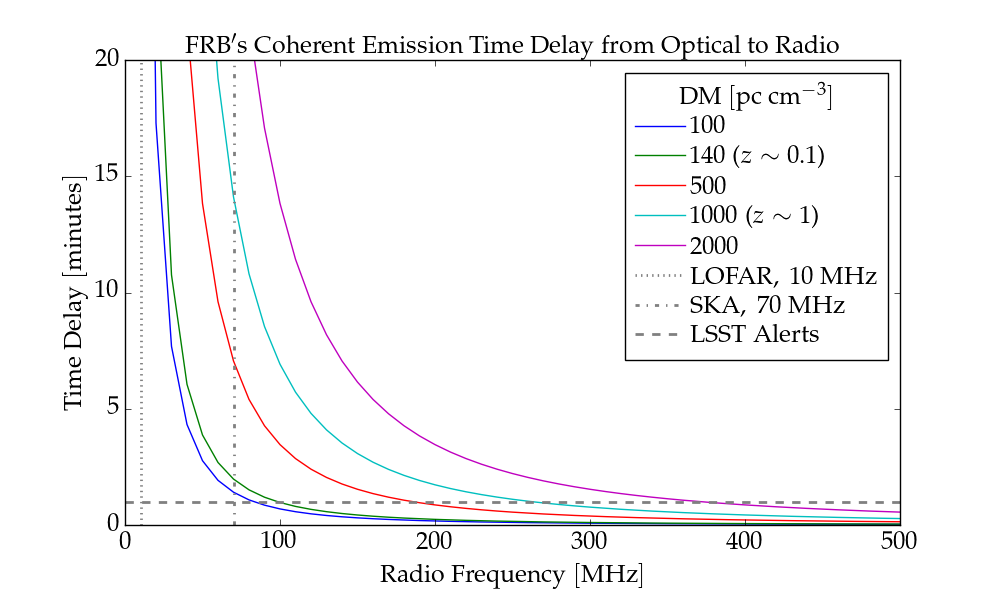
\includegraphics[width=15cm]{figures/frb_optical_delays.png}
\caption{The delay time (for coherent emission) between the arrival of the optical and radio photons due to cosmological dispersion, as a function of the frequency of the radio detector. The {\it lowest} frequency bands of the Square Kilometer Array (SKA) and the Low-Frequency Array (LOFAR) are marked with vertical dotted and dash-dotted lines, and the 1 minute timescale for LSST alert distribution with a horizontal dashed line. The delay time is $\Delta t = k_{\rm DM}\,DM\,(\nu_{\rm low}^{-2} - \nu_{\rm high}^{-2})$, where $k_{DM}=4.149$ $\rm GHz^2\ pc^{-1}\ cm^3\ ms$, ${\rm DM}$ is the dispersion measure in $\rm pc\ cm^{-3}$, $\nu$ is the low and high frequency bands of the observation, and $\Delta t$ is in $\rm ms$. We have used the range of FRB dispersion measures as observed by \cite{2018Natur.562..386S}. \label{fig:sci_frb}}
\end{center}
\end{figure}

\subsection{Young Supernovae}\label{ssec:latency_ysne}

Photometric data obtained during the first few hours to days of a supernova can constrain the progenitor radius and circumstellar material in the immediate environment, which in turn provides information about the progenitor star, its system, and its final stages of evolution before the explosion.
For example, \citet{2018Natur.554..497B} model the optical photometric data of the post-shock breakout cooling peak for a massive star's core collapse supernova to constrain the radius and mass of its outer envelope; \citet{2012ApJ...744L..17B} used the first day of photometric observations of a nearby Type Ia (thermonuclear detonation) supernova to show that their progenitor stars must be a compact degenerates; and rare ``blue bumps" in the first few days of a Type Ia supernova's light curve might betray the presence of a non-degenerate companion star \citep[e.g.,][]{2010ApJ...708.1025K,2017ApJ...845L..11H}.

For young supernovae, follow-up observations within a couple of hours are required, and the related science goals are unlikely to be impacted if the alert latency was 5--10 minutes instead of 1 minute.

\subsection{Solar System Objects}\label{ssec:latency_sso}

\textcolor{red}{MLG: in Lynne's talk on the SSSC needs for alerts brokers at the CBW in June 2019, slide 4 says that a needed broker capability was "API or other 'push' notification (e.g., trailed detections) [minutes may count]". Follow-up on the SS use case for alerts on very short timescales.}

\subsection{Stellar Variables}\label{ssec:latency_stars}

\textcolor{red}{Return to the road map or science book? Surely there must be some stellar use-cases for 1 minute alerts. E.g., microlensing peaks can be real sharp.}

\citet{2006ApJ...644L..63K}, the discovery of three $<$hour optical transients in the Deep Lens Survey (one confirmed M star and two with potentially extragalactic origin), has been invoked as motivation for the 30 second exposure times and 60 second alert production latency -- e.g., the Deep Lens Survey is referenced without citation in the LSST Science Requirements Document. More recently, \citet{2013ApJ...779...18B} searched for fast optical transients in the Pan-STARRS1 Medium-Deep Survey identified 19 fast transients: 11 M dwarf flares and 8 likely solor system objects. \citet{2018ApJ...854L..13H} searched for fast-fading transients in archival data from the Palomar Transient Factor and found 50 candidates: three GRB afterglows (\S~\ref{ssec:latency_grb}), eight artifacts, one asteroid, and 38 with red stellar counterparts identified as M dwarfs. \textcolor{red}{Their Fig 1 is a delta-mag vs. delta-time plot comparing afterglows to Mdwarf flares that shows how they can be photometrically distinguished (difference regions of that parameter space)}. \textcolor{red}{Existence of short duration M dwarf flares established; what's the science related to them?}


% Include all the relevant bib files.
% https://lsst-texmf.lsst.io/lsstdoc.html#bibliographies
\bibliography{local,lsst,lsst-dm,refs_ads,refs,books}

\end{document}
